\chapter{Decision Making}

An AI agent should be capable of making decisions. Based on what it observes, what it believes, and what it desires, the agent must determine the most beneficial action or sequence of actions to take. In many practical problems, the consequences of actions or even the “best” reachable states of the system are not known in advance. The AI agent must therefore rely on trial and error, learning from successful and failed attempts to develop an optimal policy across different scenarios.

This chapter studies decision making with AI. Markov Decision Process is discussed in detail, as it is one of the most widely used decision-making frameworks.

\section{General Introduction to Decision Making with AI}

To formulate a decision-making problem mathematically, the first step is to define the \mync{utility} (often in the form of a function) that quantifies the value of an action or system state. Decision making is essentially the process of maximizing utility. This section introduces the concept of utility and the formulation of utility functions, and how utility is used in decision making with AI.

\subsection{Utility Theory}

Intuitively, a rational AI agent should always choose the action that maximizes expected utility among all available actions. This is known as the \mync{maximum expected utility} (MEU) principle. Below, MEU is formulated as an optimization problem.

When the AI agent decides to perform an action among all the actions it can take, the system transitions from one state to another. Let the \mync{transition model} be denoted by $P(s|a,e)$, where $e$ represents the evidence or observation of the system, incorporating the agent’s awareness of its current origin state, $a$ denotes the action taken, and $s$ is the destination state. The probabilistic form of $P(s|a,e)$ captures uncertainty in the system.

The benefit of reaching a state is quantitatively described by the \mync{utility of a state} $U(s)$. The utility $U(s)$ usually includes not only the immediate reward of reaching the state $s$, but also the foreseeable future benefits that may arise from reaching $s$ as an intermediate state. For now, do not bother how $U(s)$ can be calculated. Later in Sections \ref{sec:mdp} and \ref{sec:pomdp}, the systematic calculation of $U(s)$ will be introduced.

The \mync{expected utility of action} $EU(a|e)$, given evidence $e$, over possible landing states $s_i \in S$, can be expressed by
\begin{eqnarray}
	EU(a|e) &=& \sum_{s_i \in S} P(s_i|a,e) \left(R(s_i,a,e) + U(s_i)\right) \label{eq:expected_utility}
\end{eqnarray}
where $R(s_i,a,e)$ is the reward gained by taking the action $a$ to reach $s$ given the observation $e$, and $U(s)$ the utility of state $s$. 

Given the evidence $e$, an AI agent may take one of several actions $a_i \in A$. MEU suggests that the optimal action is
\begin{eqnarray}
	a^* &=& \argmax_{a_i \in A} EU(a_i|e) \label{eq:emu}
\end{eqnarray}

An example of MEU is given by Fig.~\ref{fig:emuexp}. Consider a maze in which a robotic AI agent is randomly placed in one of several locations (blocks). Each location corresponds to a state represented by the coordinate $(x,y)$. The agent can move horizontally or vertically one step at a time. Let the utility of a state be given by its shortest distance to the goal, as shown in Fig.~\ref{fig:emuexp}. The utility, in this example, can be interpreted as the minimum turn required to reach the goal, if optimal actions are taken everywhere. To give it physical meanings, it can be the expected battery consumption of the robot to reach the goal with the most efficient route.

\begin{figure}[!htb]
	\centering
	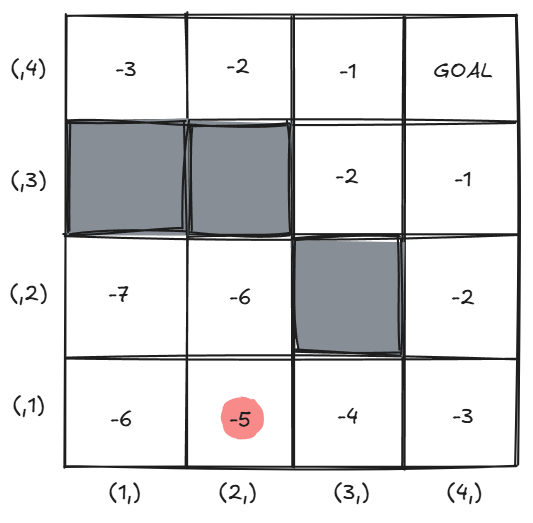
\includegraphics[width=0.5\textwidth]{./chapters/part-1/figures/emuexp.png}
	\caption{State utility map in the MEU example.}
	\label{fig:emuexp}
\end{figure}

Let $e$ represent the agent’s current location, assumed to be the red dot at $(2,1)$. The agent can take four actions, listed below along with their possible resulting states and associated probabilities:
\begin{eqnarray}
	a_1 &=& \mathrm{UP} \nonumber \\
	P((2,1)|a_1,e) &=& 0.2 \nonumber \\
	P((2,2)|a_1,e) &=& 0.6 \nonumber \\
	P((1,1)|a_1,e) &=& 0.1 \nonumber \\
	P((3,1)|a_1,e) &=& 0.1 \nonumber \\
	a_2 &=& \mathrm{LEFT} \nonumber \\
	P((2,1)|a_2,e) &=& 0.2 \nonumber \\
	P((2,2)|a_2,e) &=& 0.1 \nonumber \\
	P((1,1)|a_2,e) &=& 0.6 \nonumber \\
	P((3,1)|a_2,e) &=& 0.1 \nonumber \\
	a_3 &=& \mathrm{DOWN} \nonumber \\
	P((2,1)|a_3,e) &=& 0.7 \nonumber \\
	P((2,2)|a_3,e) &=& 0.1 \nonumber \\
	P((1,1)|a_3,e) &=& 0.1 \nonumber \\
	P((3,1)|a_3,e) &=& 0.1 \nonumber \\
	a_4 &=& \mathrm{RIGHT} \nonumber \\
	P((2,1)|a_4,e) &=& 0.2 \nonumber \\
	P((2,2)|a_4,e) &=& 0.1 \nonumber \\
	P((1,1)|a_4,e) &=& 0.1 \nonumber \\
	P((3,1)|a_4,e) &=& 0.6 \nonumber
\end{eqnarray}

Note that the outcome of an action is not deterministic. In practice, this may result from signal transmission errors or environmental uncertainty. The agent cannot move downward from its current location, so when it chooses the “DOWN” action $a_3$, it will likely remain in the same place after encountering a wall.

Using \eqref{eq:expected_utility}, the expected utility of $a_1$ can be computed as
\begin{eqnarray}
	EU(a_1|e) &=& 0.2 \times (-5) + 0.6 \times (-6) + 0.1 \times (-6) + 0.1 \times (-4) \nonumber \\
	&=& -5.6 \nonumber
\end{eqnarray}
Similarly, $EU(a_2|e) = -5.6$, $EU(a_3|e) = -5.1$, and $EU(a_4|e) = -4.6$. Therefore, according to \eqref{eq:emu}, the rational decision is to take action $a_4$, i.e., move “RIGHT.”

In this example, all states $s_i$, transition probabilities $P(s_i|a,e)$, and utilities $U(s_i)$ are assumed known. This is rarely the case in practical problems. Sections~\ref{sec:mdp} and~\ref{sec:pomdp} will introduce methods for estimating or learning these quantities.

\begin{mdframed}
	\noindent \textbf{Are there alternatives to expected utility?}
	
	The expected utility of an action is calculated using \eqref{eq:expected_utility}. An AI agent using \eqref{eq:expected_utility} and \eqref{eq:emu} to make decisions behaves rationally. 
	
	However, can we base decision making on other measures of utility? For example, consider the worst-case utility:
	\begin{eqnarray}
		WU(a|e) &=& \min\{U(s_i)\,|\,P(s_i|a,e) > 0\} \nonumber
	\end{eqnarray}
	Instead of maximizing expected utility, could we maximize worst-case utility?
	
	This question concerns the definition of a rational agent. To formalize this, the following \mync{axioms of utility theory} are defined:
	\begin{itemize}
		\item \textbf{Orderability.} For any two actions $a_1$ and $a_2$, exactly one of the following statements must hold: “$a_1$ is preferred over $a_2$,” “$a_1$ and $a_2$ are indifferent,” or “$a_2$ is preferred over $a_1$.” Thus, any two actions can be ranked.
		\item \textbf{Transitivity.} If $a_1$ is preferred over $a_2$ and $a_2$ is preferred over $a_3$, then $a_1$ must be preferred over $a_3$.
		\item \textbf{Continuity.} For three actions $a_1$, $a_2$, and $a_3$, where $a_1$ is preferred over $a_2$ and $a_2$ over $a_3$, there exists a probability $p$ such that a compound action $a_{1,3,p,1-p}$ (which randomly chooses $a_1$ with probability $p$ and $a_3$ with $1-p$) is indifferent to $a_2$.
		\item \textbf{Substitutability.} If $a_1$ and $a_2$ are indifferent and $a_3$ is any action, then for any $p$, the compound actions $a_{1,3,p,1-p}$ and $a_{2,3,p,1-p}$ must be indifferent.
		\item \textbf{Monotonicity.} If $a_1$ is preferred over $a_2$, then for compound actions $a_{1,2,p_1,1-p_1}$ and $a_{1,2,p_2,1-p_2}$, if $p_1 > p_2$, then $a_{1,2,p_1,1-p_1}$ is preferred over $a_{1,2,p_2,1-p_2}$.
		\item \textbf{Decomposability.} Compound actions can be nested or decomposed. For example, if $a_{1,2,p,1-p}$ is a compound action and $a_2$ is itself a compound action $a_2 = a_{21,22,q,1-q}$, then $a_{1,2,p,1-p}$ is indifferent to $a_{1,21,22,p,(1-p)q,(1-p)(1-q)}$.
	\end{itemize}
	
	Let $U(a|e)$ (or simply $U(a)$) denote the utility of action $a$. The specific form of $U(a)$, whether it represents expected utility or another valid measure, is acceptable as long as the following conditions are satisfied:
	\begin{itemize}
		\item $U(a)$ must exist for every action.
		\item $U(a)$ must reflect preference: if $U(a_1) > U(a_2)$, then $a_1$ is preferred over $a_2$; if $U(a_1) = U(a_2)$, they are indifferent.
		\item The preferences reflected by $U(a)$ satisfy the axioms of utility theory.
	\end{itemize}
	
	For any utility $U(a)$ satisfying these criteria, the utility of a compound action composed of actions $a_1, \dots, a_n$ with corresponding probabilities $p_1, \dots, p_n$ is given by
	\begin{eqnarray}
		U(a_{1,2,\dots,n,p_1,p_2,\dots,p_n}) &=& \sum_i p_i U(a_i) \nonumber
	\end{eqnarray}
	
	Note that the utility function is not unique. For instance, given a utility function $U(a)$,
	\begin{eqnarray}
		U'(a) &=& \alpha U(a) + \beta, \quad \alpha > 0 \nonumber
	\end{eqnarray}
	is also a valid utility function.
	
\end{mdframed}

\subsection{Utility Function}

The utility of an action $U(a|e)$, for example $EU(a|e)$ as in \eqref{eq:expected_utility}, is an instance of a \mync{utility function} that maps actions to real numbers. As noted earlier, the expected utility formulation is not the only valid approach consistent with the axioms of utility theory. Nonetheless, it is the most widely used and is employed in the \myabb{Markov Decision Process}{MDP}, which will be introduced in Sections~\ref{sec:mdp} and~\ref{sec:pomdp}. For the remainder of this chapter, unless otherwise specified, we consider expected utility as defined in \eqref{eq:expected_utility}.

The expected utility of an action depends on the transition model $P(s|a,e)$ and the state utility $U(s)$. State utility typically includes both its immediate reward and the anticipated future utility obtainable from using that state as an intermediate step. For example, in chess, each board configuration represents a state. Only the final checkmate state provides immediate utility, but intermediate states possess utility as they contribute to eventual victory.

The computation of utility functions for actions and states is often referred to as \mync{preference elicitation}. Different models have different ways of defining and calibrating utility functions. As far as this notebook concerns, utility calculation of MDP will be introduced in details in Sections~\ref{sec:mdp} and \ref{sec:pomdp}. In the remainder of this section, factors and good practices of determine utilities, especially immediate reward of a state, are discussed. Notice that anticipated future utilities of states and utilities of actions can often be derived from the immediate rewards of states and the transition models.

While the detailed calculation of utilities varies by task and will be addressed later, some general principles for assigning utility values are useful and they are given below.
\begin{itemize}
	\item Although utility is relative, it is often helpful to define global upper and lower bounds, where the lower bound represents “immediate loss” and the upper bound represents “goal achieved.”
	\item In many real-world problems, utility is expressed in monetary terms (financial gain or cost). Rewards and penalties of various types are converted to monetary values and normalized by a scaling factor.
	\item Decision makers may differ in risk preference. Risk-averse and risk-seeking agents can have different utility functions even under identical circumstances.
	\item Mathematically derived utility functions sometimes contradict human intuition, as humans are not always rational and do not always conform to the axioms of utility theory.
\end{itemize}

An \mync{influence diagram} or \mync{decision network} represents the structure of a utility function. It is a graphical model illustrating the relationships between utility, its contributing attributes, and the factors influencing those attributes, as well as the entities responsible for making decisions. Understanding this structure helps decision makers identify which factors influence outcomes and should be considered when determine the utility values.

An example is shown in Fig.~\ref{fig:decisionnetworkexp}, where a decision network assists a buyer in choosing a house. Here, the utility function depends on three attributes—location, construction quality, and price—each determined by several underlying factors. The entity ``buyer'' controls these attributes, selecting actions (purchase choices) that maximize utility.

\begin{figure}[!htb]
	\centering
	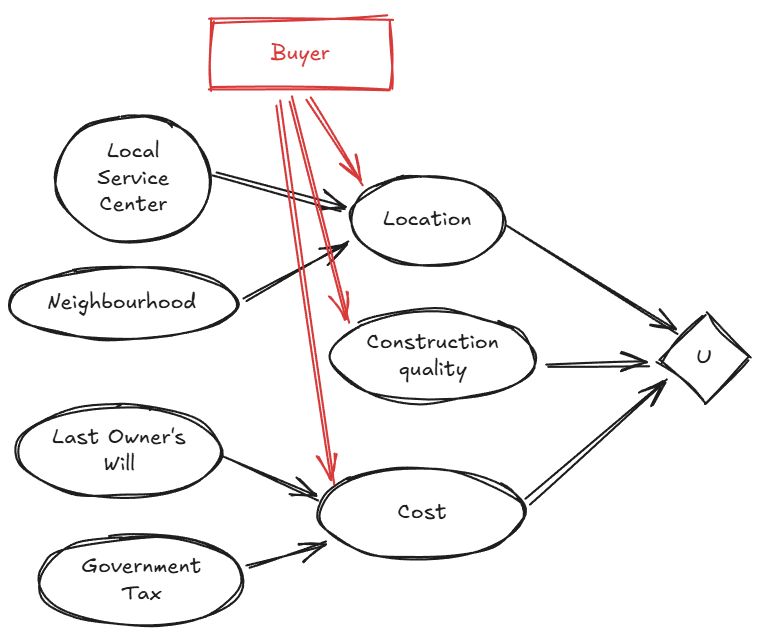
\includegraphics[width=0.75\textwidth]{./chapters/part-1/figures/decision_network_exp.png}
	\caption{A simple decision network in which a buyer must decide which house to purchase.}
	\label{fig:decisionnetworkexp}
\end{figure}

\section{Markov Decision Process} \label{sec:mdp}

Up to this point, we have introduced the basic principles of decision making. In summary, utility must be defined for each action, and it should be designed to satisfy the axioms of utility theory so that the agent behaves rationally. In practice, the utility of system states is specified, and the utility of an action can be derived from state utilities and the transition model. The decision network helps formulate the utility of a state. The action with the highest expected utility is often regarded as optimal, and this principle is known as MEU.

Equations \eqref{eq:expected_utility} and \eqref{eq:emu} are a realization of the above, with Fig.~\ref{fig:emuexp} providing an example. In that example, the utilities of all states and the transition model are assumed known, which is not always true in reality. While the example in Fig.~\ref{fig:emuexp} is simple, real-world problems are often more complex. Consider a similar setting to Fig.~\ref{fig:emuexp}, except that
\begin{itemize}
	\item The possible system states are unknown in advance; that is, the size, shape, and boundary of the maze are initially unknown, and the agent must explore by trial and error.
	\item The utility of each state is unknown in advance; the agent does not know how far each state is from the goal and thus cannot use that information as guidance until it discovers the goal through exploration.
	\item The transition model is unknown in advance. The agent does not know which actions will move it up, left, down, or right, and the effect of each action may depend on the current state. In the extreme case, the set of available actions differs across states.
\end{itemize}
These factors substantially increase the difficulty of the problem.

MDP provides a framework to tackle such problems. Through MDP, the agent can learn via trial and error to calibrate state utilities and the transition model. There will be failures in which the agent falls into traps and successes in which it finds the goal (or goals). Through repeated trials and reinforcement learning, it can eventually determine what action to take at each position to avoid traps and reach goals as efficiently as possible.

This section and the next Section~\ref{sec:pomdp} study MDP and discuss the calibration of state utilities and the transition model.

\subsection{General Review of MDP}

A \mync{Markov Decision Process} (MDP) refers to the following decision-making problem formulation:
\begin{itemize}
	\item It defines state, which is a minimal set of information that reflects the current status of the system. 
	\item It defines transmission models, which describe the relationship between the current state, the action taken, and the resulting next state. The transition model is often given by the stochastic model $P(s|s\textprime,a)$ (essentially the same as $P(s|a,e)$ in \eqref{eq:expected_utility}, where current-state information is incorporated into the evidence $e$). The transition model is Markovian, i.e., it depends only on the current state and action, not on the full history.
	\item Actions are chosen sequentially until a time horizon is reached or a goal state is achieved.
	\item A utility function is defined for the agent. The utility is an accumulation of rewards that agent gains by traveling among states. For each travel, the agent get some reward which is determined by the destination state, the action taken, the origin state, or all of them jointly.
	\item The objective is to determine the policy at each state. The policy maps each state to the best action that maximizes the expected agent utility.
\end{itemize}

Depending on whether the agent has the full picture of the current state, the MDP formulations can be divided into two types, namely fully observable MDP and \myabb{partially observable MDP}{POMDP}. This section studies fully observable while the next Section ~\ref{sec:pomdp} studies POMDP. 

\begin{mdframed}
	\noindent \textbf{Known MDP versus Fully Observable MDP}
	
	Notice that a fully observable MDP assumes the agent always knows its current state but does not necessarily know the transition model or reward function. It also does not need to know all possible states in advance. These quantities can be learned or calibrated through trial and error using reinforcement learning.
	
	If a fully observable MDP also has complete knowledge of all transition models at every state and all possible rewards for each state–action pair, it becomes a \mync{known MDP}. Figure~\ref{fig:emuexp} illustrates an example of a known MDP, where the maze layout and the goal position are both clearly marked. In this case, the agent does not need to explore, and it can compute the optimal policy before taking any action.
	
	Now consider a similar scenario in which the robot does not know the size or shape of the maze, nor the positions of walls or goals in advance. This means the agent does not know the set of reachable states, the transition model (i.e., which actions are possible in each state and their outcomes), or the reward function. It still, however, knows its current position. In this case, the system remains a fully observable MDP, but it is no longer a known MDP.
	
	\vspace{0.1in}
	\noindent \textbf{How to Define the State}
	
	A natural question that follows is how to determine what information should be included in the state. After all, if we were to define the transition model or reward function themselves as part of the state (which we should not), a fully observable MDP would degenerate into a known MDP.
	
	The principle is that in an MDP, the state must be Markovian: it must contain the minimum information required to compute the probabilistic result of an action and the associated reward, assuming the transition and reward models are known. The agent should not need to refer to historical states or actions for these calculations. Importantly, the state should contain all variables necessary for the transition and reward models to be formulated in a stationary manner.
	
	The following examples illustrate how to decide what information should be included in the state.
	
	Consider a robot navigating a maze. It knows its current position, represented by coordinates, but it does not know the locations of walls. The following cases are considered:
	
	\begin{itemize}
		\item Case 1: Finding the goal.
		
		In this case, the state should include only the robot’s current location. With the current position as the state, a stationary transition model can describe how each action leads to a resulting state and what reward the agent receives if it reaches the goal or a trap. The agent may not initially know which positions correspond to walls or traps, but that information is stationary in the sense that when the agent revisits the same location, the same outcomes apply. Through repeated trials, the agent can learn these relationships.
		
		\item Case 2: Exploring as many unique locations as possible within a time horizon.
		
		Here, it is insufficient for the state to include only the current location. Although the transition model can still describe how actions lead to new positions, this information alone cannot determine the reward, since the reward depends on whether the robot visits new locations or revisits old ones.
		
		Defining the state as the current location together with the total number of moves made is still insufficient, because the reward depends on the set of unique locations visited, not just the count of moves.
		
		If the state is defined as the current location and the set of previously visited unique locations, the reward can indeed be computed. However, the transition model must also be able to determine the next state. Without knowledge of whether the next position has been visited, it cannot update the number of visited unique locations correctly.
		
		Therefore, to preserve the Markov property, the state must include the current location along with the complete history of all previously visited locations. Only then can both the transition model and the reward function be expressed in a stationary form.
		
		\item Case 3: Finding the goal under changing environmental conditions.
		
		In this scenario, the positions of walls change according to certain external conditions (e.g., time, temperature, or other factors). The wall configuration directly affects the transition model. If the state includes only the robot’s current location, the transition model becomes non-stationary, violating the MDP assumption (see note below). 
		
		The state must therefore include the external conditions that influence the maze layout, ensuring that the transition model remains stationary.
	\end{itemize}
	
Note: In practice, even if the transition model or reward function of a system is non-stationary (for example, changing with time or other external conditions), the problem can always be reformulated as a stationary MDP by augmenting the state with all relevant variables that cause the non-stationary, such as time or system mode. Therefore, in this notebook, it is assumed without loss of generality that the transition model and the reward function of an MDP are stationary. This assumption is standard in most theoretical formulations and practical implementations of MDP.

\end{mdframed}

\subsection{Reward, Utility, and Policy}

The following concepts are introduced or revisited in this section:
\begin{itemize}
	\item Reward
	\item Utility, Utility of State, Utility of Action
	\item Policy, Utility of Policy, Optimal Policy
\end{itemize}
Concepts previously introduced are here re-emphasized in the specific context of MDP.

\vspace{0.1in}
\noindent \textbf{Reward}
\vspace{0.1in}

A reward is the instantaneous gain or loss obtained by taking an action or reaching a state. Rewards are assumed to be stationary. If rewards vary dynamically (e.g., with time or environmental conditions), the factor causing this variation should be incorporated into the MDP state so that the reward function remains stationary.  

Rewards can take several common forms as follows.
\begin{itemize}
	\item Reward by reaching a state, $R(s)$
	
	In some problems, the agent gains a reward or penalty upon reaching a particular state. The previous state or the action taken to reach that state is irrelevant.  
	For example, in the robot-in-a-maze problem, the robot receives a positive reward when it reaches the goal and a negative reward when it reaches a trap. The reward depends only on the destination state, not on the path taken.
	
	\item Reward by taking an action, $R(a)$
	
	In other problems, rewards are associated with performing actions. For example, a robot navigating a maze may receive a small negative reward for each move to represent battery consumption.  
	
	In general, a reward can depend on both the origin and destination states, and the action taken. Such cases are denoted by $R(s, a, s\textprime)$, where the first $s$ is the origin state, $a$ the action, and $s\textprime$ the destination state.
\end{itemize}



\vspace{0.1in}
\noindent \textbf{Utility, Utility of State, Utility of Action}
\vspace{0.1in}

Utility differs from reward. A reward represents an immediate benefit gained at a specific step, while utility is a cumulative or comprehensive measure of value that reflects the long-term desirability of a state or an action. In other words, reward is instantaneous, whereas utility captures the expected future rewards achievable from a given state or action. Utility is typically derived or calibrated from rewards but embodies the notion of potential benefit rather than immediate gain.

The following example illustrates the distinction. Consider a game of chess. A reward is obtained only when the game ends in checkmate, positive for the winner and negative for the loser. However, checkmate cannot occur on the first move. If snapshots of the board are taken after each round, the probability of winning gradually increases for one player, from about $50\%$ at the start to nearly $100\%$ at checkmate. Although the actual reward is given only at the end, every board configuration during the game has a certain utility. The closer a configuration is to a winning position, the more likely the reward will be gained from that configuration, hence the higher its utility.

The calculation of utility from rewards is introduced as follows. Before the introduction, it is worth mentioning the two types of MDPs with finite and infinite maximum allowed number of actions, as they are treated slightly differently when calculating utility.

\begin{itemize}
	\item Finite horizon
	
	There is a fixed time horizon $N$. After $N$ actions, the game ends and no further utility is accumulated. The goal is to maximize total utility within these $N$ steps.
	
	In this case, although the transition model and reward function can remain stationary, the optimal policy may be non-stationary and vary with the remaining time. Suppose the agent returns to the same state after $k<N$ actions. With only $N-k$ steps left, the optimal policy may differ from what it would have been initially when all $N$ steps were available.
	
	The optimal policy can be made stationary by augmenting the remaining time horizon into the state. When that value becomes zero, no more rewards can be received.
	
	\item Infinite horizon
	
	The game has no explicit time limit, and it terminates only when certain conditions are met—for example, when the agent reaches particular terminal states.
	
	In this case, the optimal policy is typically stationary. The optimal action at a given state remains fixed and does not depend on when the state is reached. Care must be taken in defining the utility function, however, because if rewards are unbounded or poorly scaled, the agent may loop indefinitely to accumulate infinite utility, rendering the problem ill-defined.
\end{itemize}

In whichever the case, assume the following scenario. An agent starts with zero utility or reward. It receives $R_0$ right away at the current state $s_0$. It performs action $a_{0,1}$ to transform state from $s_0$ to $s_1$. The action awards a reward $R_{0,1}$. After reaching state $R_1$, it receives a reward $R_1$. It then performs $a_{0,2}$ to transform state from $s_1$ to $s_2$ and it gains $R_{1,2}$. After landing at state $s_2$, it receives $R_2$, and so on. Stationary rewards and transition models are assumed.

The utility the agent collects can be formulated as a collective of rewards as follows.
\begin{eqnarray}
	U &=& R_0 + R_{0,1} + \gamma \left(R_1 + R_{1,2} + \gamma \left(R_2 + R_{2,3} + \gamma(\ldots)\right)\right) \label{eq:rewardtoutility}
\end{eqnarray}
where $0 < \gamma \leq <1$ is known as the \mync{discount factor}. The discount factor has at least two purposes. When $\gamma < 1$ is used, it guarantees that the utility is bounded even in a infinite horizon MDP, so that the agent cannot gain infinite utility by circulating around a few state. It also reflects a widely adopted assumption in finance, where a future reward of the same value is often less worthy than an immediate reward.

Notice that one may formulate \eqref{eq:rewardtoutility} as follows
\begin{eqnarray}
	U &=& R_0 + \gamma \left(R_{0,1} + R_1 + \gamma \left(R_{1,2} + R_2 + \gamma(\ldots)\right)\right) \nonumber
\end{eqnarray}
where the action reward $R_{a,b}$ is treated the same way as $R_{b}$ when applying the discount factor. This expression lives in a parallel world of \eqref{eq:rewardtoutility} and everything should work just alright so long as everything is consistent. Nevertheless, \eqref{eq:rewardtoutility} is more commonly adopted, where we assume that the reward of an action is received together with the origin state reward, not the destination state reward.

Following the spirit in \eqref{eq:rewardtoutility}, the utility of a state can be recurrently defined as follows.
\begin{eqnarray}
	U(s) &=& R(s) + \max_{a\in A(s)}\left(\sum_{s_i \in S} P(s_i|s,a)\left(R(s,a,s_i) + \gamma U(s_i)\right)\right) \label{eq:bellman}
\end{eqnarray}
where $s$ is the state of interest, $U(s)$ the utility of state $s$, $R(s)$ the reward received immediately when reaching the state, $a\in A(s)$ all the actions that can be taken at the state, $s_i \in S$ all the states or all the states reachable from $s$ with action $a$, $P(s_i|s,a)$ the probability of reaching $s_i$ from $s$ with action $a$, $R(s,a,s_i)$ the immediate reward obtained by action $a$ transforming state from $s$ to $s_i$, and $U(s_i)$ the utility of state $s_i$. Equation \eqref{eq:bellman} is known as the \mync{Bellman equation}. Notice that in Bellman equation, it is assumed that the agent is rational and always takes the action that maximizes the utility.

Bellman equation \eqref{eq:bellman} can be used recurrently to calculate the utility of states. This is known as the value iteration, which will be introduced in more details in Section~\ref{sec:mdpvalue}.

The utility of an action $a$ at state $s$ is given by
\begin{eqnarray}
	U(a|s) &=& \sum_{s_i \in S} P(s_i|s,a)\left(R(s,a,s_i) + \gamma U(s_i)\right) \label{eq:bellmanaction}
\end{eqnarray}
which describes the expected return from taking an action at a state (under a policy). Equation \eqref{eq:bellmanaction} also known as the \mync{Q-function}. Q-function \eqref{eq:bellmanaction} is related to utility of state \eqref{eq:bellman} as follows.
\begin{eqnarray}
	U(s) &=& R(s) + \max_{a\in A(s)} U(a|s) \nonumber
\end{eqnarray}
 
Equation \eqref{eq:bellman} and \eqref{eq:bellmanaction} reveals the correlation between the utility of a state and the utility of an action. The utility of state $s$ is the reward of arriving the state plus the maximum utility of action among all the actions the agent can take from the state.

\vspace{0.1in}
\noindent \textbf{Policy, Utility of Policy, Optimal Policy}
\vspace{0.1in}

A policy refers to a ``rule book'' that says what action to take at each and every state. A policy is often denoted by
\begin{eqnarray}
	\pi(s): && s \rightarrow a \label{eq:mdppolicy}
\end{eqnarray}
as a map from the state $s$ and $a$. The utility of a policy, giving an initial state, can be calculated by \eqref{eq:rewardtoutility} where the rewards are those collected rewards by an agent following that policy. With stationary reward and transmission model and with a properly chosen discount factor, the utility of a policy is always bounded. 

Among all the probable policies, the policy that gives the highest utility is known as the optimal policy, often denoted by $\pi^*(s)$. It is fairly easy to prove that with stationary reward and transmission model, the optimal policy is also stationary, meaning that when the system is at the same state, the optimal policy should always suggest the same action to do. Hence in the scope of MDP, we only studies stationary policy.

When the optimal policy is applied, the agent choose the action with the maximum utility from \eqref{eq:bellmanaction}, i.e.,
\begin{eqnarray}
	\pi^*(s) = \argmax_{a\in A(s)} \sum_{s_i \in S} P(s_i|s,a)\left(R(s,a,s_i) + \gamma U(s_i)\right) \label{eq:mdpoptpolicy}
\end{eqnarray}
When there are multiple actions that give the same largest utility, the agent randomly choose one action from them.

\subsection{Value Iteration} \label{sec:mdpvalue}

To get the optimal policy $\pi^*(s)$ given by \eqref{eq:mdpoptpolicy}, the key is to get the utility of state $U(s)$. The Bellman equation \eqref{eq:bellman} provides a way to recursively calculate the utility of state as follows.
\begin{eqnarray}
	U_{i+1}(s) &\leftarrow& R(s) + \max_{a\in A(s)}\left(\sum_{s_i \in S} P(s_i|s,a)\left(R(s,a,s_i) + \gamma U_i(s_i)\right)\right) \label{eq:bellmanupdate}
\end{eqnarray}
which is known as the \mync{value iteration} of MDP.

The following example is given to demonstrate the use of Bellman equation to update the utility of states.

\begin{shortbox}
\Boxhead{A Robot in a Maze with Dynamic Rewards and Traps}

Place a robot in a $4\times 4$ maze. 

The robot can move in all directions for one block, or stay at its current space in each round of action. The robot cannot move outside the maze. This defines $9$ actions for the robot if it is in the center area of the maze, $6$ actions if it is beside an edge, and $4$ sections if it is at the corner. When the robot makes an action, there is a probability of $P$ that the command is interpreted correctly and the robot will behave accordingly. There is a probability of $1-P$ that the robot fails to interpret the command, in which case it will randomly select an action from what it can do.

Some locations of the maze are assigned with rewards or penalties. There are two sets of different rewards configurations and they switch every $5$ actions. The two setups are given in Fig.~\ref{fig:valueiterationexp}. The reward map is known in advance.

The robot is able to sense its location and also the time, meaning that it knows not only the current reward setup, but also the future reward map swaps.

The target is to design an MDP and calculate the utility of state using Bellman update. 

\end{shortbox}

\begin{figure}[!htb]
	\centering
	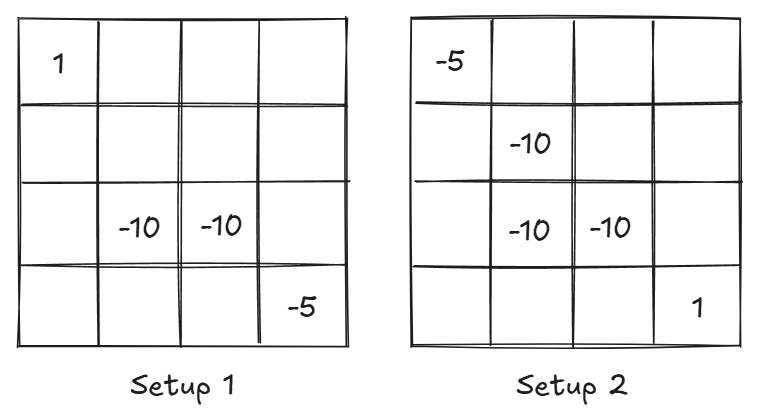
\includegraphics[width=0.75\textwidth]{./chapters/part-1/figures/valueiterationexp.png}
	\caption{Reward in the example, where the reward change periodically over time.}
	\label{fig:valueiterationexp}
\end{figure}

Define the state. Notice that the rewards are determined jointly by the location and time cycle. To make the reward stationary, the time cycle information must be included in the MDP state definition. The two reward setups swap every $5$ actions. Therefore, the reward configuration cycle is $10$ actions. There are a total of $4\times 4\times 10=160$ states ($4\times 4=16$ the distinct location of the robot, and $10$ the time index in the reward cycle).

For the convenience, let $x$ a $3\times 1$ vector that can be used to denote the states. The first element $x(1)\in \{1,2,3,4\}$ is the horizontal axis, the second element $x(2)\in \{1,2,3,4\}$ the vertical axis, and the third element $x(3) = \{1,\ldots,10\}\}$ the time index.

Define the transition model. In this example, different states have different available actions. When the robot is at the edge or at the corner, it will have less moving options. For simplicity, only two actions from two states as follows are given as examples below. The rest actions can be formulated similarly.

Consider state $x=[2,2,1]$. This is one of the center area of the maze, and the robot can move $9$ directions from this state (one of them being stay where it is). A total of $9$ actions can be defined for this state. Take ``up'' action as an example. The destination state and the probability for this action is given below.
\begin{eqnarray}
	P\left([1,1,2]|[2,2,1], \mathrm{up}\right) &=& \dfrac{1-P}{9} \nonumber \\
	P\left([1,2,2]|[2,2,1], \mathrm{up}\right) &=& \dfrac{1-P}{9} \nonumber \\
	P\left([1,3,2]|[2,2,1], \mathrm{up}\right) &=& \dfrac{1-P}{9} \nonumber \\
	P\left([2,1,2]|[2,2,1], \mathrm{up}\right) &=& \dfrac{1-P}{9} \nonumber \\
	P\left([2,2,2]|[2,2,1], \mathrm{up}\right) &=& \dfrac{1-P}{9} \nonumber \\
	P\left([2,3,2]|[2,2,1], \mathrm{up}\right) &=& \dfrac{1-P}{9} + P \nonumber \\
	P\left([3,1,2]|[2,2,1], \mathrm{up}\right) &=& \dfrac{1-P}{9} \nonumber \\
	P\left([3,2,2]|[2,2,1], \mathrm{up}\right) &=& \dfrac{1-P}{9} \nonumber \\
	P\left([3,3,2]|[2,2,1], \mathrm{up}\right) &=& \dfrac{1-P}{9} \nonumber
\end{eqnarray} 
There are a total of $9$ possible destination state for this action at this state. Notice that the time index increases by $1$ then the action is performed. Consider another state $x=[4,4,10]$. This is a corner state, and the robot can move only $4$ directions from this state. A total of $4$ actions are defined. Take ``left'' as an example. The destination state and the probability for this action is given below.
\begin{eqnarray}
	P\left([3,3,1]|[4,4,10], \mathrm{left}\right) &=& \dfrac{1-P}{4} \nonumber \\
	P\left([3,4,1]|[4,4,10], \mathrm{left}\right) &=& \dfrac{1-P}{4} + P \nonumber \\
	P\left([4,3,1]|[4,4,10], \mathrm{left}\right) &=& \dfrac{1-P}{4} \nonumber \\
	P\left([4,4,1]|[4,4,10], \mathrm{left}\right) &=& \dfrac{1-P}{4} \nonumber
\end{eqnarray} 
The time index loops to $1$ after taking the action.

The reward is formulated as follows. There is no reward for actions $R(s, a, s\textprime)$, and only rewards for certain states $R(s)$ as follows.
\begin{eqnarray}
	R([1,4,i]) &=& 1, i=1,...,5 \nonumber \\
	R([2,2,i]) &=& -10, i=1,...,5 \nonumber \\
	R([3,2,i]) &=& -10, i=1,...,5 \nonumber \\
	R([4,1,i]) &=& -5, i=1,...,5 \nonumber \\
	R([1,4,i]) &=& -5, i=6,...,10 \nonumber \\
	R([2,2,i]) &=& -10, i=6,...,10 \nonumber \\
	R([2,3,i]) &=& -10, i=6,...,10 \nonumber \\
	R([3,2,i]) &=& -10, i=6,...,10 \nonumber \\
	R([4,1,i]) &=& -10, i=6,...,1 \nonumber
\end{eqnarray}

Set discount rate to be $\gamma=0.8$ and success rate of action to be $P=0.9$.

Looping over the entire $160$ states using \eqref{eq:bellmanupdate} is known as one iteration. After $42$ iterations, the utility of the state converges. Fig~\ref{fig:valueiterationexp2} gives some of the results.

\begin{figure}[!htb]
	\centering
	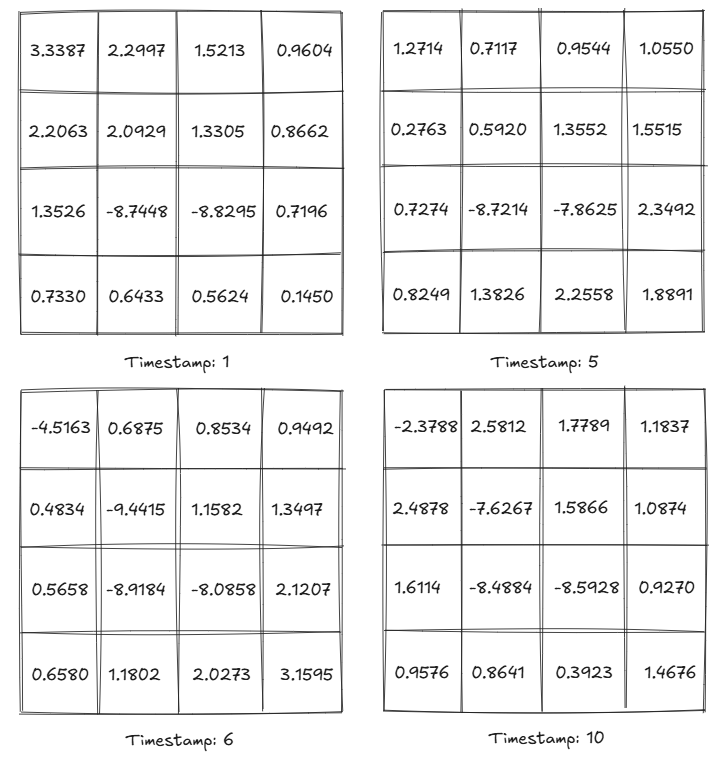
\includegraphics[width=\textwidth]{./chapters/part-1/figures/valueiterationexp2.png}
	\caption{Converged utility of state at timestamps $1$,$5$,$6$ and $10$.}
	\label{fig:valueiterationexp2}
\end{figure}

Some highlights are as follows.
\begin{itemize}
	\item The agent tries to stay far away from the ``traps''. There is a fail rate for a move. If the agent stay adjacent to a trap, it may fall into the trap by accident. For safety, the agent prefers to stay or move around at safer areas far away from the traps.
	\item The utility of state is a function of timestamps. Notice that although the reward configurations at timestamp $1$ and $5$ are identical, the utility of states are different. At timestamp $5$, the agent is aware that the reward configuration is going to change, and it is preparing for it. There are several motivations. The original reward sweet point will be a trap, and the agent wants to stay away from it. There is a discount factor, which motivates the agent to move to the new reward point as quickly as possible.
\end{itemize}

When the reward configuration and transition model are known and stationary, we can use value iteration to calculate the utility of state. With utility of state known, it is straight forward to decide the optimal policy using \eqref{eq:mdpoptpolicy}.

It can be proved that if infinite iteration is used, Bellman update will converge to the unique global optimum. Proof is not given here.

\subsection{Policy Iteration}

\mync{Policy iteration} is an alternative way of finding the optimal policy given the reward configuration and transition model. Unlike the value iteration where the utility of the state is first calculated, in policy iteration, it is started with assuming a policy $\pi^0(s)$ which is not necessarily optimal.

With that $\pi^0(s)$, the utility of state can be calculated using \eqref{eq:rewardtoutility}. With the utility of state calculated, use \eqref{eq:mdpoptpolicy} to revise the policy to get $\pi^1(s)$. Repeat the above steps iteratively until the utility of state and the policy converge.

Policy iteration and value iteration should lead to the same result. It is reported that sometimes policy iteration is easier to implement.

\subsection{MDP Online Reinforcement Learning}

Both value iteration and policy iteration assume known reward configuration and transition model, which is often not true. In practice, the agent needs to explore and find the transition model associated with each action at each state as well as the rewards received from each action or state. Inspired by policy iteration, the following \mync{Q-Learning} algorithm can be used.

\begin{enumerate}
	\item In the beginning when there is no information of reward and transition model, initialize utility of state \eqref{eq:bellman} with $0$ for all states. Initialize the Q-function with $0$ for all actions at all states.
	\item Let the agent freely transition from the current state until the end of the session, either when it reaches the goal, runs into a trap, or after certain time. Notice that the action with the largest utility is not necessarily selected. It uses a exploit-explore model instead, which will be introduced later.
	\item For each state visited in the trail, update the Q-function of the actions taken together with the utility of the state as follows, from the first state to the last state.
	
	\begin{eqnarray}
		U_{k+1}(a|s) &\leftarrow& U_k(a|s) + \alpha_k\left(R(s,a,s_i) + \gamma U_k(s_i)\right) \label{eq:qlearningupdate} \\
		U_{k+1}(s) &\leftarrow& R(s) + \max_{a\in A(s)} U_{k+1}(a|s) \nonumber
	\end{eqnarray}

\end{enumerate}
where steps 2 and 3 are repeated so that the agent keeps learning from different trails, until the agent has gained enough information about each and every action and each and every state, and no further learning is required.

In \eqref{eq:qlearningupdate}, $\alpha_k$ should fulfill the following criteria, so that the Q-function and utility of state converge to the optimum.
\begin{eqnarray}
	&& \sum_{k=0}^{\infty} \alpha_k^2 < \infty \nonumber \\
	&& \sum_{k=0}^{\infty} \alpha_k \rightarrow \infty \nonumber
\end{eqnarray}
which implies that until everything converges, the agent must keep learning. An example of $\alpha_k$ can be $\alpha_k = 1/k \alpha_0$ with a finite $\alpha_0$.

As mentioned earlier, for the agent to keep learning, it should not always stay in its comfort zone by running only the estimated optimal policy. It is encouraged to always explore new actions that is not the best action under existing estimated optimal policy. It is important to maintain a proper exploit-explore balance.

The \mync{$\epsilon$-greedy exploration} model is recommended. In the $k$th trail, for each action the agent is taken, it has a $1-\epsilon_k$ probability of choosing the optimal action under the current estimated optimal policy, and a $\epsilon_k$ probability of choosing a random action, regardless of its Q-function value. The value of $\epsilon_k$ decreases as more and more trails carry out, so that the model will perform more conservative as the learned information accumulates. A common choice is $\epsilon = 1/k$.

Q-Learning is similar with value iteration or policy iteration, except that it is model-free. It is assumed that the reward configuration and transition model are unknown. It uses trails and reinforcement learning to update the utility of actions and utility of states by exploring the different states and transitions of the system.

\section{Partially Observable MDP} \label{sec:pomdp}

\mync{Partially Observable Markov Decision Process}[POMDP] refers to the case where the agent is not always clear which state it is in. Imagine in the example given by Fig~\ref{fig:emuexp}, the agent has no sense of its location in coordinate, but can detect how many walls it is adjacent to. The problem then becomes a typical POMDP. 

POMDP differs from fully observable MDP in several aspects. Though the spirit remains the same where the decision is made based on a Markov process, many details in the execution needs to be adjusted. Details are introduced in this section.

\subsection{Belief of State}

The agent, in this case, has a \mync{belief of state} often denoted by
\begin{eqnarray}
	b(s) &=& \left[p_1, \ldots, p_n\right] \nonumber
\end{eqnarray}
where $n$ is the total number of state and $p_i$ the belief of the agent currently in state $i$. One can think of $b(s)$ as a way to denote the state. The agent makes decisions based on $b(s)$.

The evidence $e$ is the measurement available to the agent. The probability $P(e|s)$ associates the state belief with the evidence. The agent can adjust its belief as follows. Let $b(s)$ be the agent's initial belief. The agent takes action $a$, and after that it observes $e$. The new belief becomes
\begin{eqnarray}
	b\textprime(s\textprime) = \alpha P(e|s\textprime) \sum_{s} P(s\textprime|s,a)b(s) \nonumber
\end{eqnarray}
where $\alpha$ is used for probability normalization so that $\sum b_i(s) = 1$ is ensured. The decision making is Markovian just like the fully observable MDP, where the optimal action depends on only the current belief of state $b(s)$. It does not depend on past states, and it does not depend on actual state.

The biggest challenge is that the $b(s)$ is a group of probability, and hence continuous and has infinite values. For example, the policy $\pi(s)$ (now $\pi(b)$) will be difficult to define, as if it were done in the conventional manner, there will be infinite possibilities. For instance, we cannot assign an action for $b(s) = [0.5,0.5]$ and another action for $b(s) = [0.501, 0.499]$. Also, the transition model which is used to be $P(s\textprime|s,a)$, is now $P(b\textprime|b,a)$ with $b$ a continuous vector.

In the remainder of the section, it is introduced how POMDP defines the transition model and optimal policy in the context of belief of state.

\subsection{Transition Model with Belief of State}

The transition model of actual state $P(s\textprime|s,a)$ and the evidence and actual state correlation $P(e|s)$ are used to derive the transition model of state of belief $P(b\textprime|b,a)$ as follows.
\begin{eqnarray}
	P(b\textprime|b,a) &=& \sum_{e}P(b\textprime|e,a,b)P(e|a,b) \nonumber \\
	&=& \sum_{e}P(b\textprime|e,a,b)\sum_{s\prime}P(e|s\textprime) \sum_{s}P(s\textprime|s,a)b(s) \nonumber
\end{eqnarray}
where
\begin{eqnarray}
	P(e|a,b) &=& \sum_{s\prime}P(e|s\textprime)P(s\textprime|a,b) \nonumber \\
	&=& \sum_{s\prime}P(e|s\textprime) \sum_{s}P(s\textprime|s,a)b(s) \nonumber
\end{eqnarray}

\subsection{Value Iteration and Optimal Policy with Belief of State}

\subsection{POMDP Online Reinforcement Learning}

\section{Multi-attribute Utility Function}

To this point, we have been assuming that all the attributes that affect utility can converted and put on the same scale. When maximizing the utility, only that single figure is considered. However, this is not always true in the reality. For example, consider personal protective equipment design. In practice, there is always a chance that the protection fails. It will take infinite money to make the equipment infinitely safe. To maximize the utility, we need to put financial cost and human life on the same scale, which is difficult and can be immoral.

A problem whose outcomes are characterized by two or more attributes that cannot be easily converted into a single figure are handled by \mync{multi-attribute utility theory}. There are several ways to handle the situation, and they are briefly introduced as follows.

In the heat map approach, the actions are converted into coordinates in a hyper space where each dimension representing an attribute. A heat map is constricted, representing the safe and dangerous zones in the hyper space. Actions inside the safe zone are selected.

In the statistic dominance approach, we investigate the chance that an action may perform better than any other actions in every aspects. The action that statistically more likely to dominant (perform better than other actions in all attributes) is selected.

Sometimes the attributes follow joint distribution. We can set a lower bound for one of the attributes, hence reducing the problem to a single-attribute problem. That attribute is used to formulate the utility function. Consider the earlier personal protective equipment example. The more expensive the gear, the more likely it is safe. The safety and the cost form a positively correlated joint distribution, where each sample in the distribution is an action. We can set a lower bound for safety requirements, for example, safety probability of $99.999\%$, and reduce the problem to a single attribute problem where we find the action with the minimum financial cost that guarantees the safety probability.

\section{Game Theory}

Multi-agent control system.